\section{Langkah-Langkah Percobaan}
\begin{enumerate}
    \item Kabel LAN digunakan untuk menghubungkan laptop ke router, serta menghubungkan satu router ke router lainnya guna membentuk jaringan yang saling terintegrasi
    \item Login dilakukan menggunakan MAC address, kemudian router di-reset terlebih dahulu melalui aplikasi Winbox untuk mengembalikannya ke pengaturan awal sebelum konfigurasi dilakukan
    \begin{figure}[H]
        \centering
        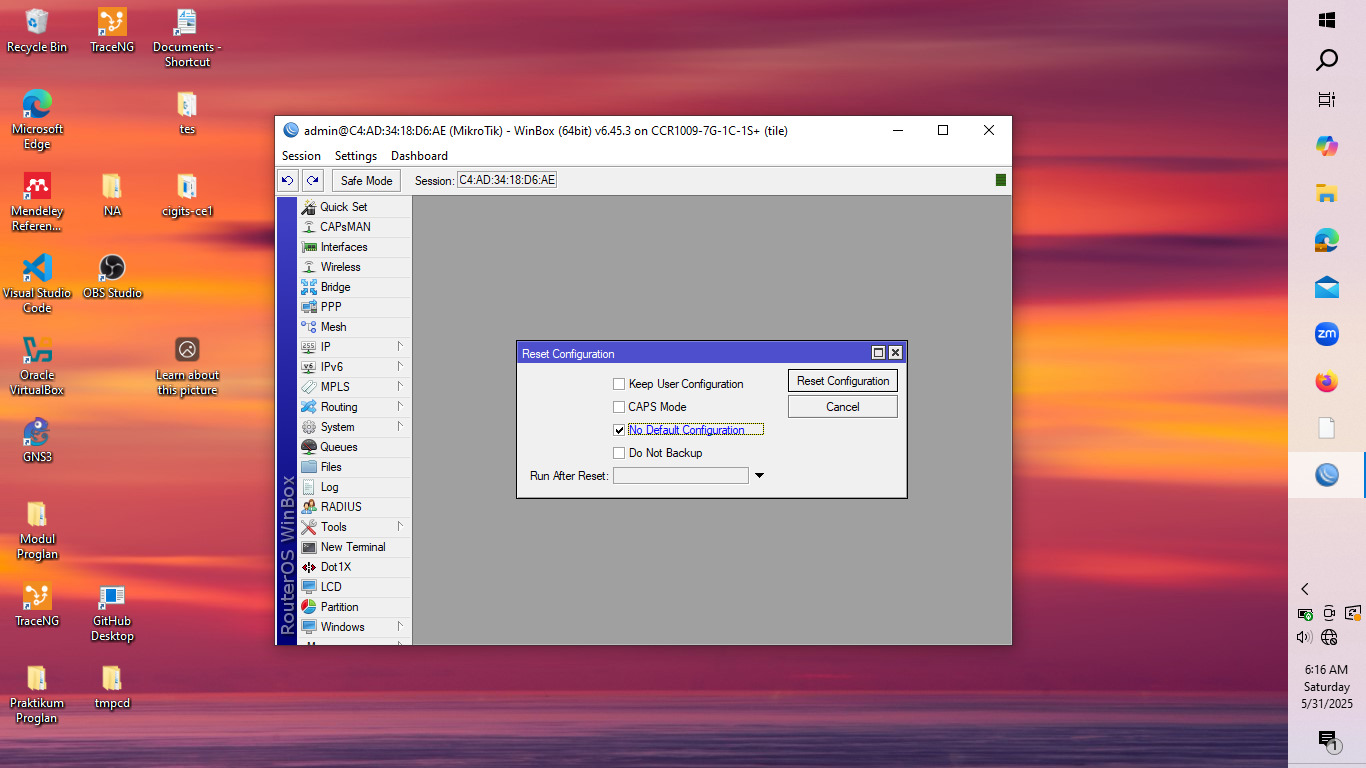
\includegraphics[width=0.5\linewidth]{P1/img/gambar1.jpeg}
        \caption{Mereset konfigurasi router melalui antarmuka Winbox.}
        \label{fig:reset-router}
    \end{figure}
    \item Menkonfigurasi Router A sebagai DHCP Client
    \begin{figure}[H]
        \centering
        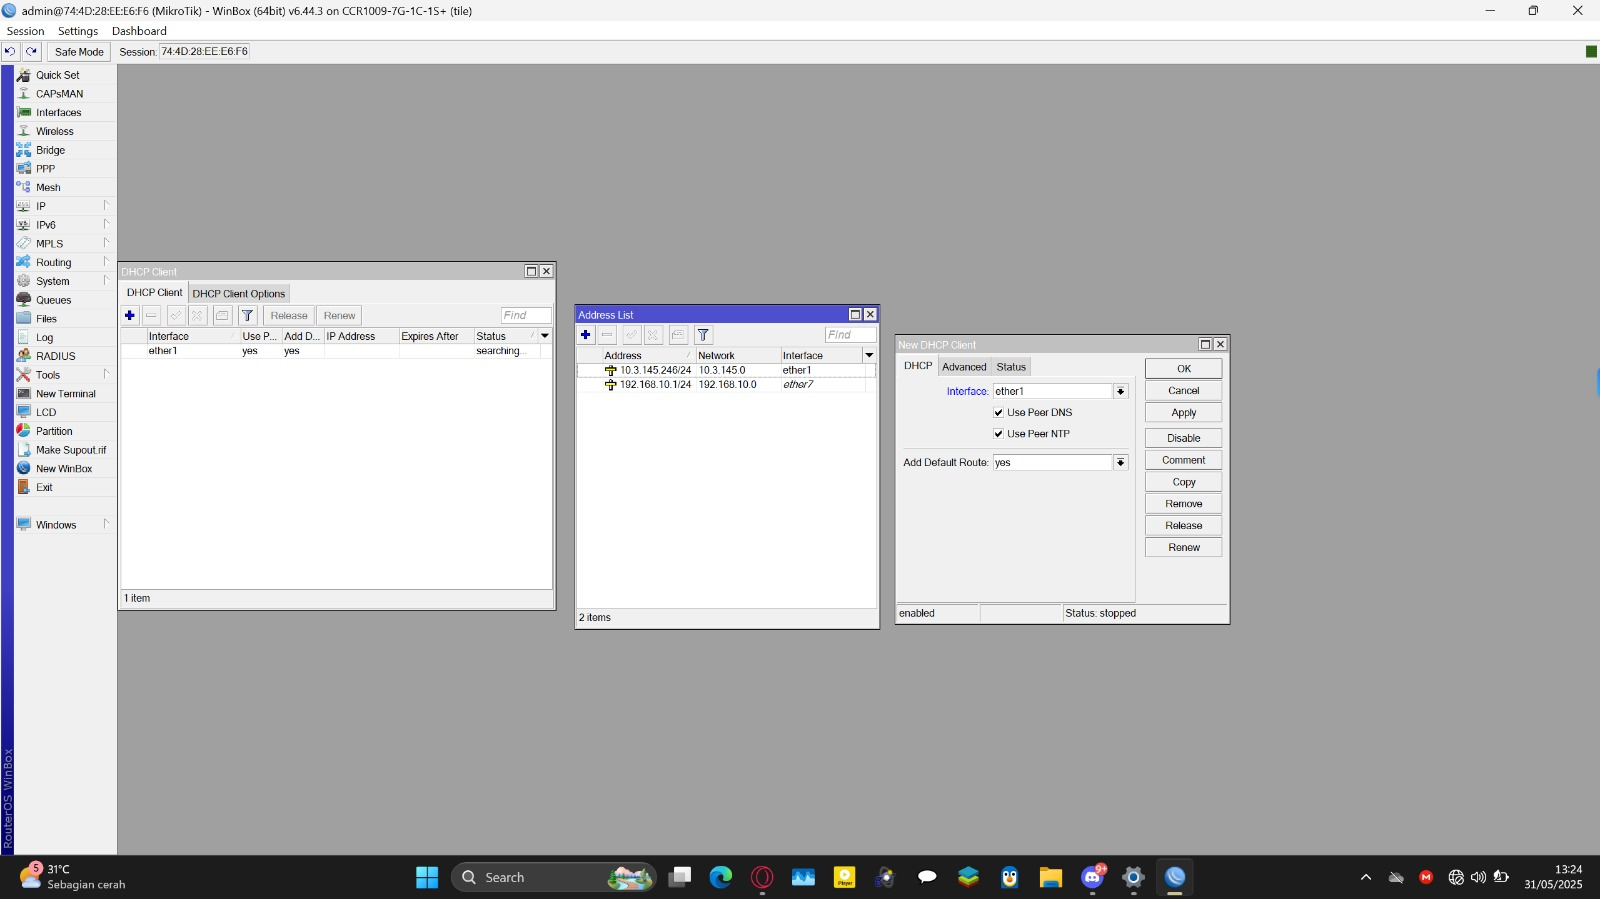
\includegraphics[width=0.5\linewidth]{P1/img/gambar2.jpeg}
        \caption{Melakukan konfigurasi DHCP Client di perangkat Router A}
        \label{fig:DHCP-router-A}
    \end{figure}
    \item Memasukkan alamat IP ke interface ether7
    \begin{figure}[H]
        \centering
        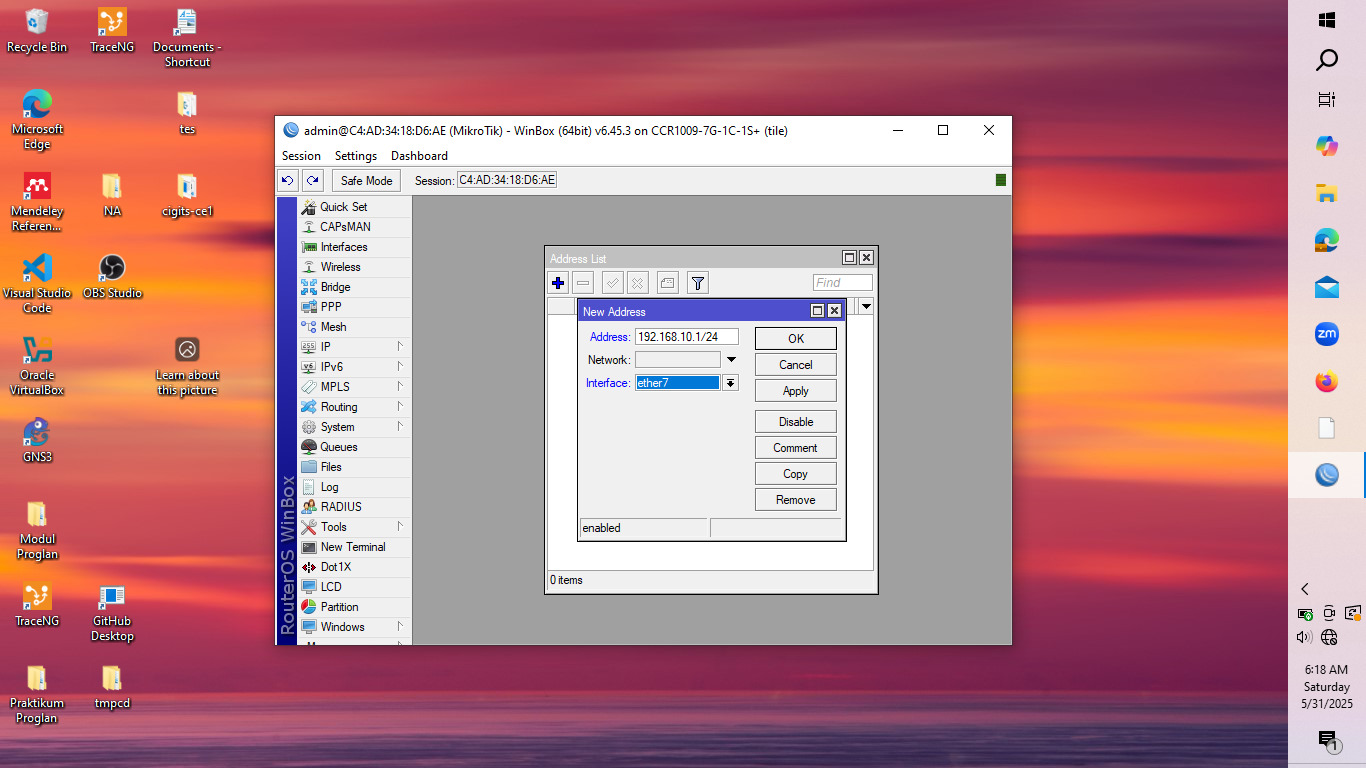
\includegraphics[width=0.5\linewidth]{P1/img/gambar3.jpeg}
        \caption{Mengatur IP address pada interface ether7}
        \label{fig:menambahkan-ip-ether7}
    \end{figure}
    \item Terapkan konfigurasi DHCP server di Mikrotik
     \begin{figure}[H]
        \centering
        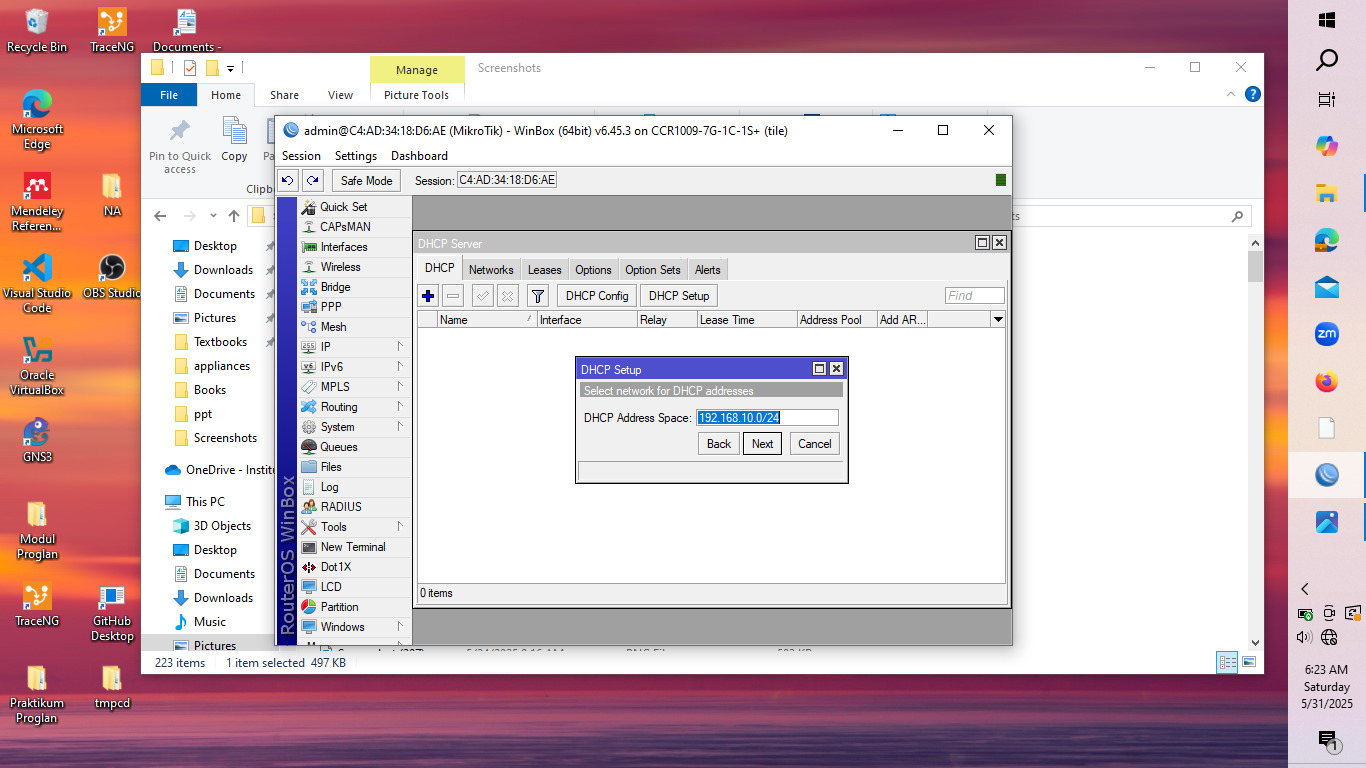
\includegraphics[width=0.5\linewidth]{P1/img/gambar4a.jpeg}
        \caption{Menetapkan konfigurasi DHCP server pada Mikrotik}
        \label{fig:mengkonfigurasikan-dhcp-server-mikrotik}
    \end{figure}

    \begin{figure}[H]
        \centering
        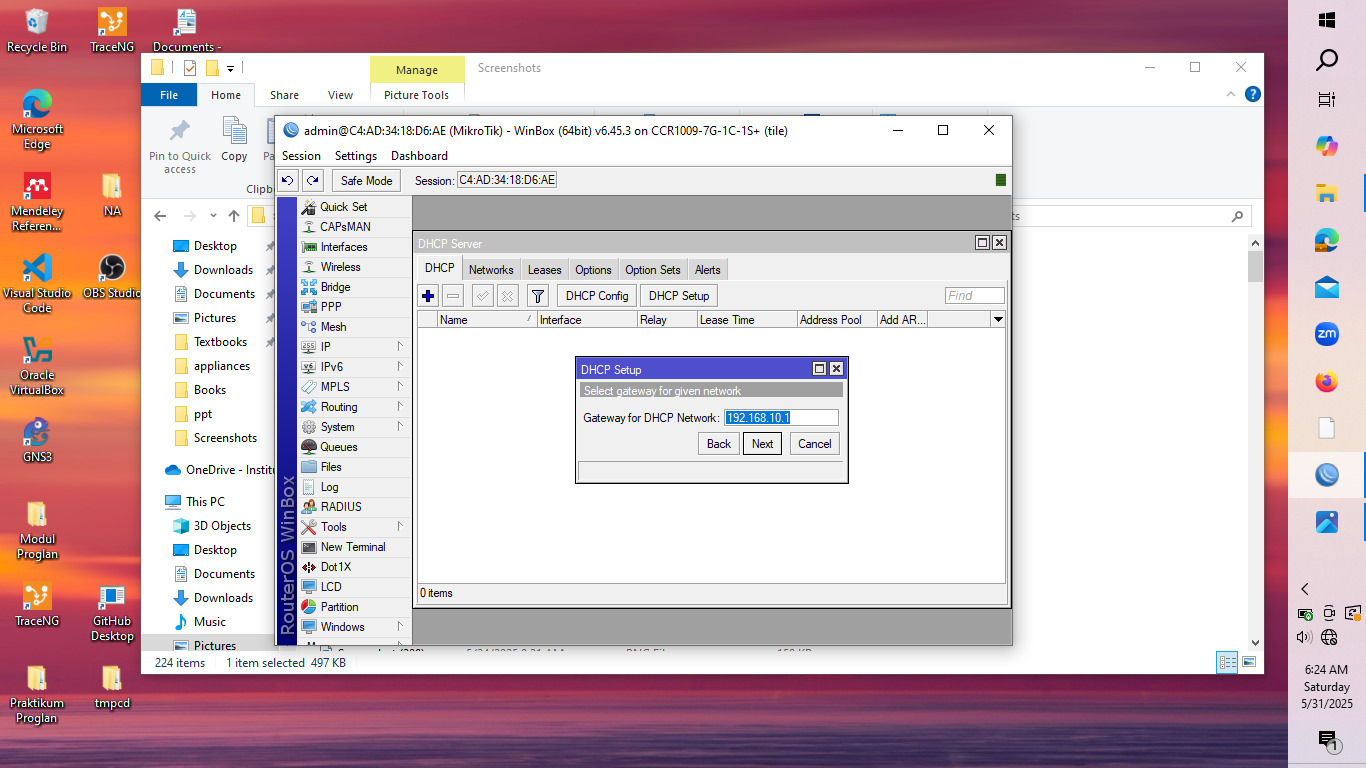
\includegraphics[width=0.5\linewidth]{P1/img/gambar4b.jpeg}
        \caption{Menetapkan konfigurasi DHCP server pada Mikrotik}
        \label{fig:mengkonfigurasikan-dhcp-server-mikrotik}
    \end{figure}

    \begin{figure}[H]
        \centering
        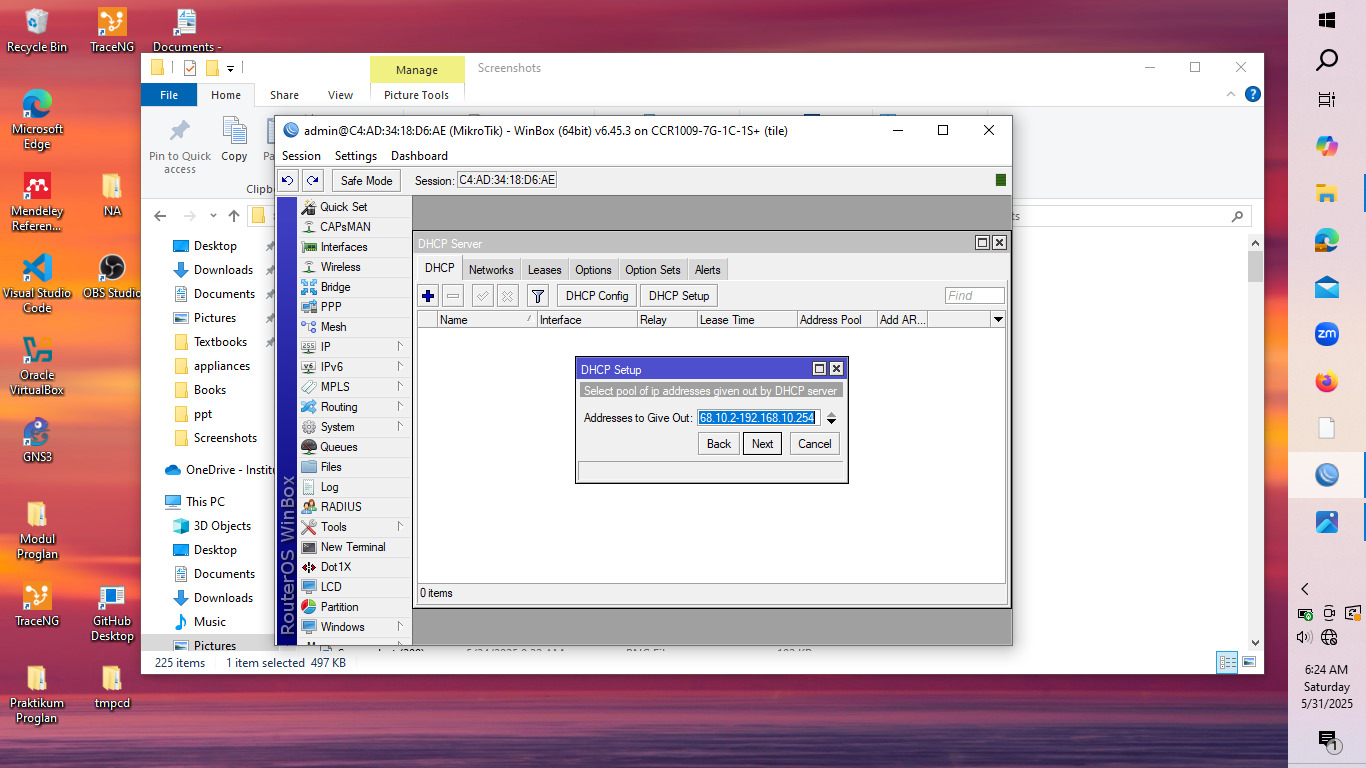
\includegraphics[width=0.5\linewidth]{P1/img/gambar4c.jpeg}
        \caption{Menetapkan konfigurasi DHCP server pada Mikrotik.}
        \label{fig:mengkonfigurasikan-dhcp-server-mikrotik}
    \end{figure}
    
    \begin{figure}[H]
        \centering
        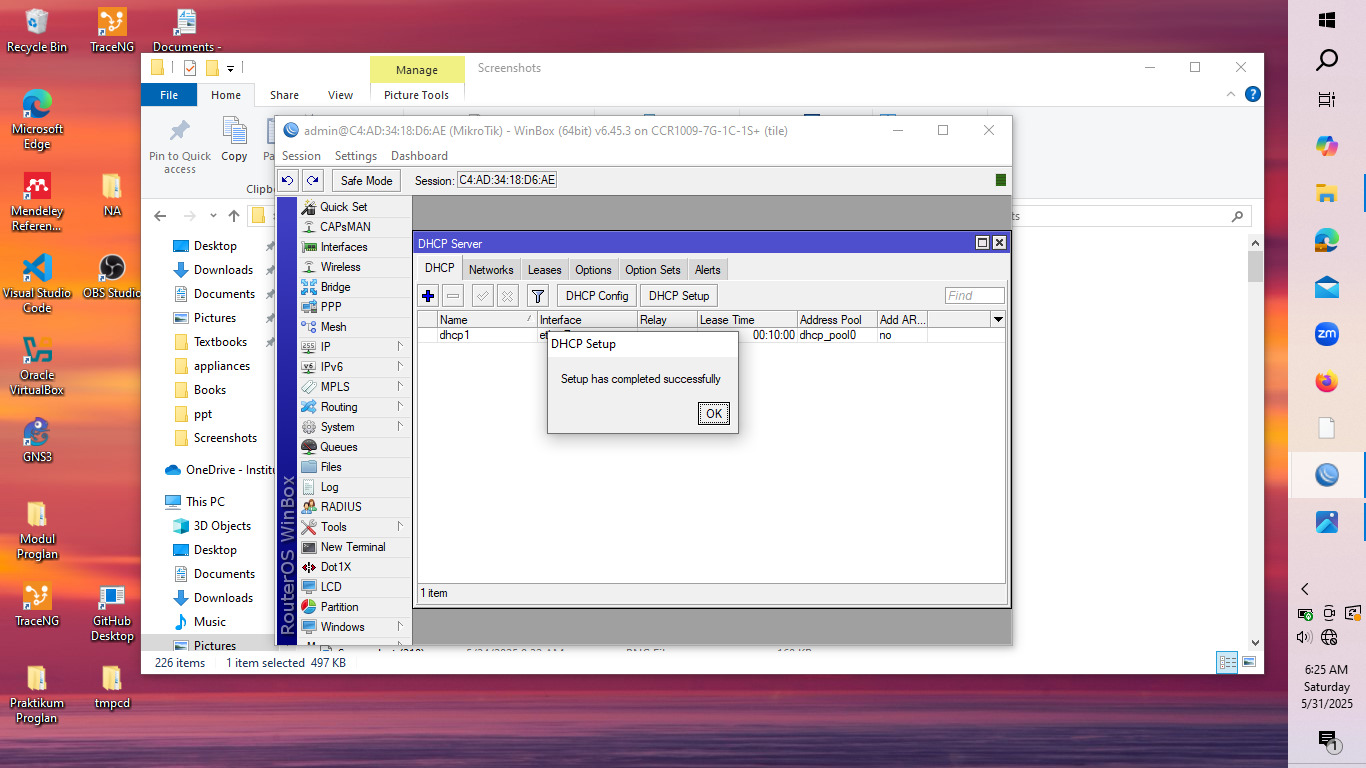
\includegraphics[width=0.5\linewidth]{P1/img/gambar4d.jpeg}
        \caption{Menetapkan konfigurasi DHCP server pada Mikrotik.}
        \label{fig:mengkonfigurasikan-dhcp-server-mikrotik}
    \end{figure}
    
    \item Lakukan konfigurasi NAT
    \begin{figure}[H]
        \centering
        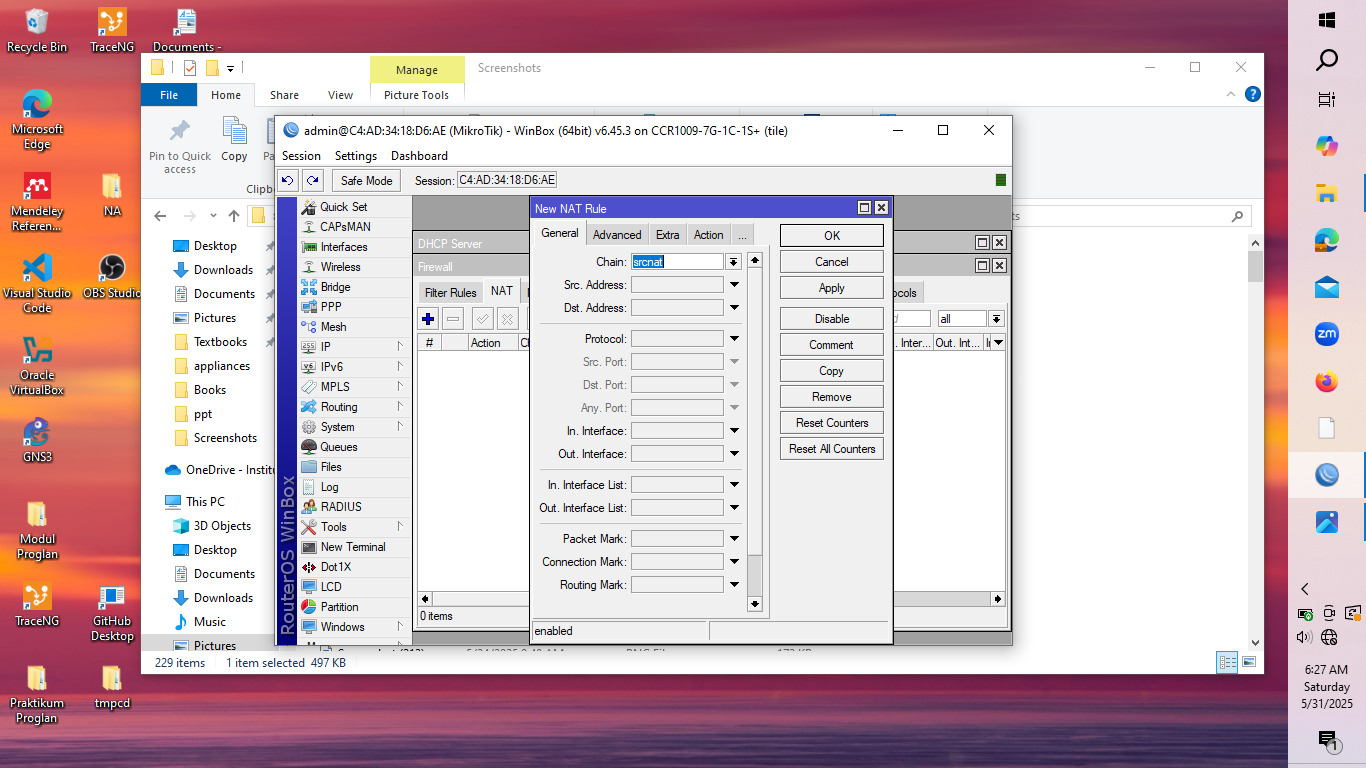
\includegraphics[width=0.5\linewidth]{P1/img/gambar5a.jpeg}
        \caption{Menerapkan konfigurasi NAT di sistem}
        \label{fig:mengkonfigurasikan-NAT}
    \end{figure}

    \begin{figure}[H]
        \centering
        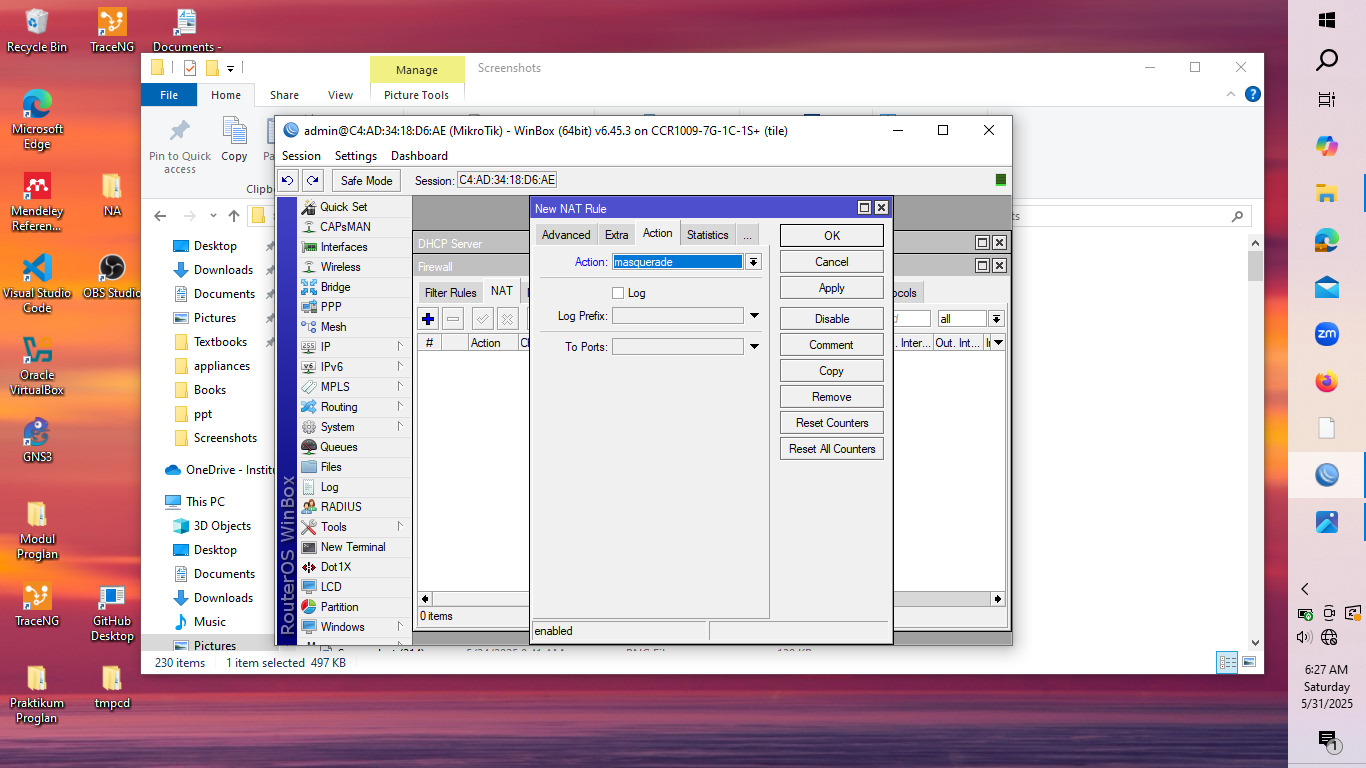
\includegraphics[width=0.5\linewidth]{P1/img/gambar5b.jpeg}
        \caption{Menerapkan konfigurasi NAT di sistem}
        \label{fig:mengkonfigurasikan-NAT}
    \end{figure}
    \item Setelah itu, lakukan pengaturan pada firewall.
    \begin{figure}[H]
        \centering
        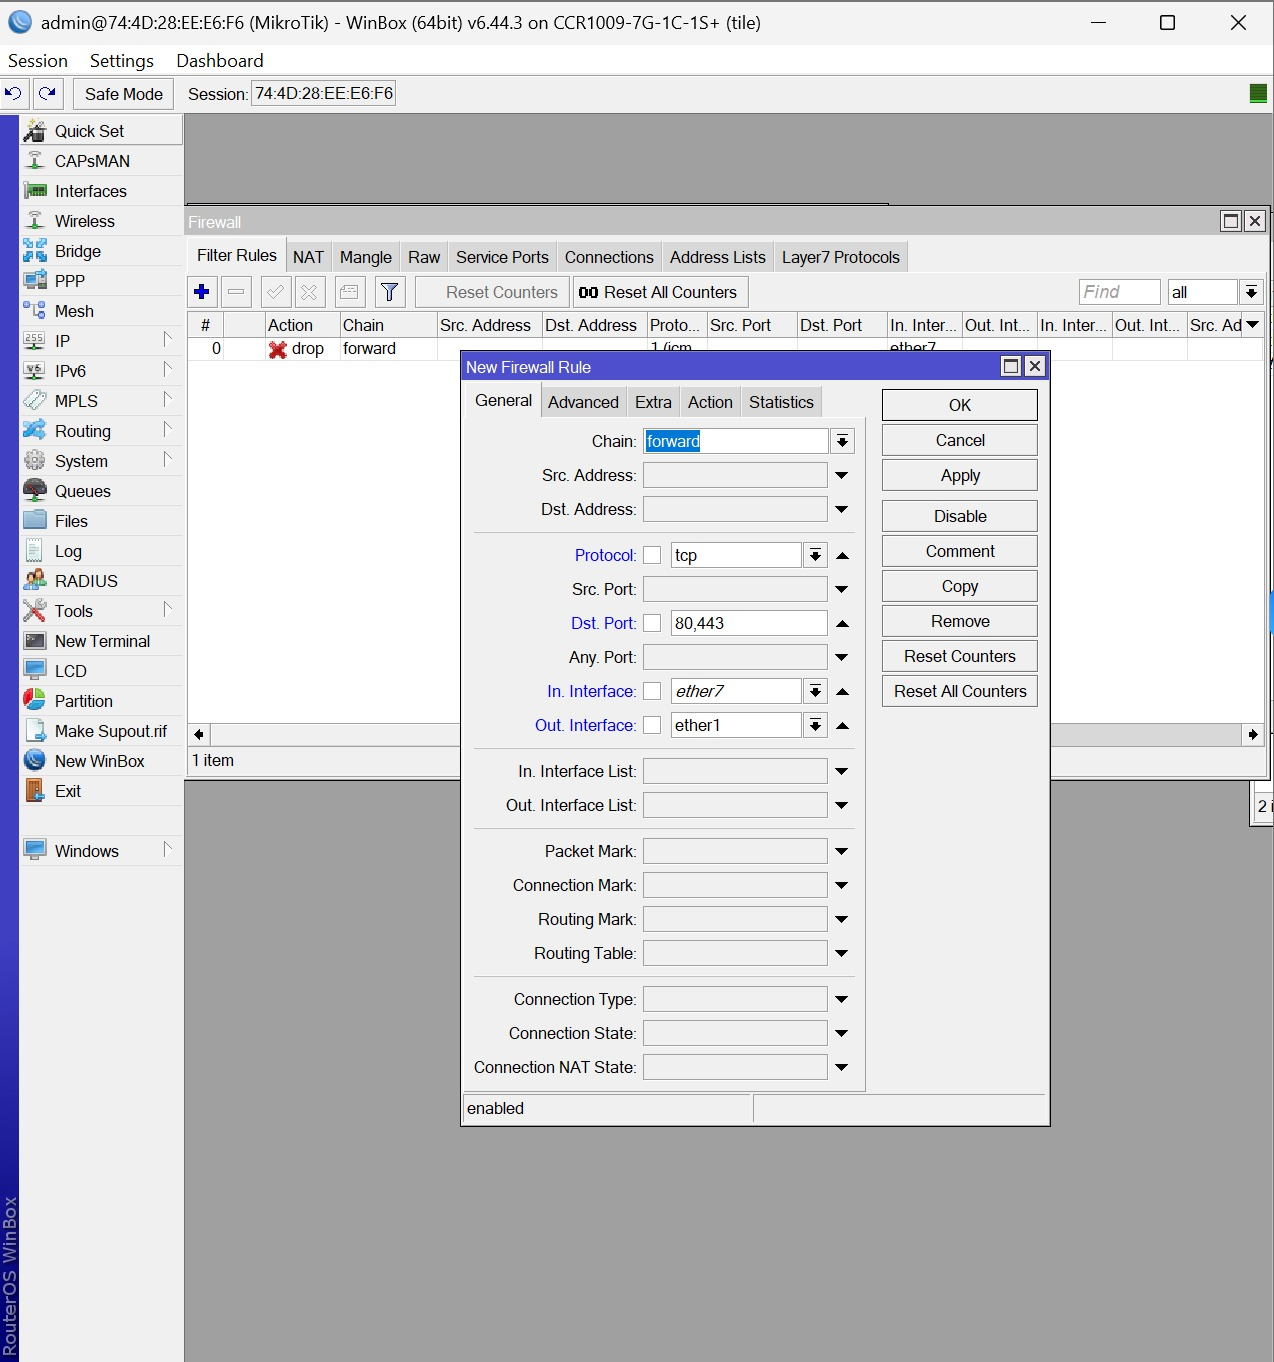
\includegraphics[width=0.5\linewidth]{P1/img/gambar6.jpeg}
        \caption{Menerapkan konfigurasi firewall}
        \label{fig:mengkonfigurasikan-firewall}
    \end{figure}
    \item Melakukan konfigurasi Bridge pada router B 
    \begin{figure}[H]
        \centering
        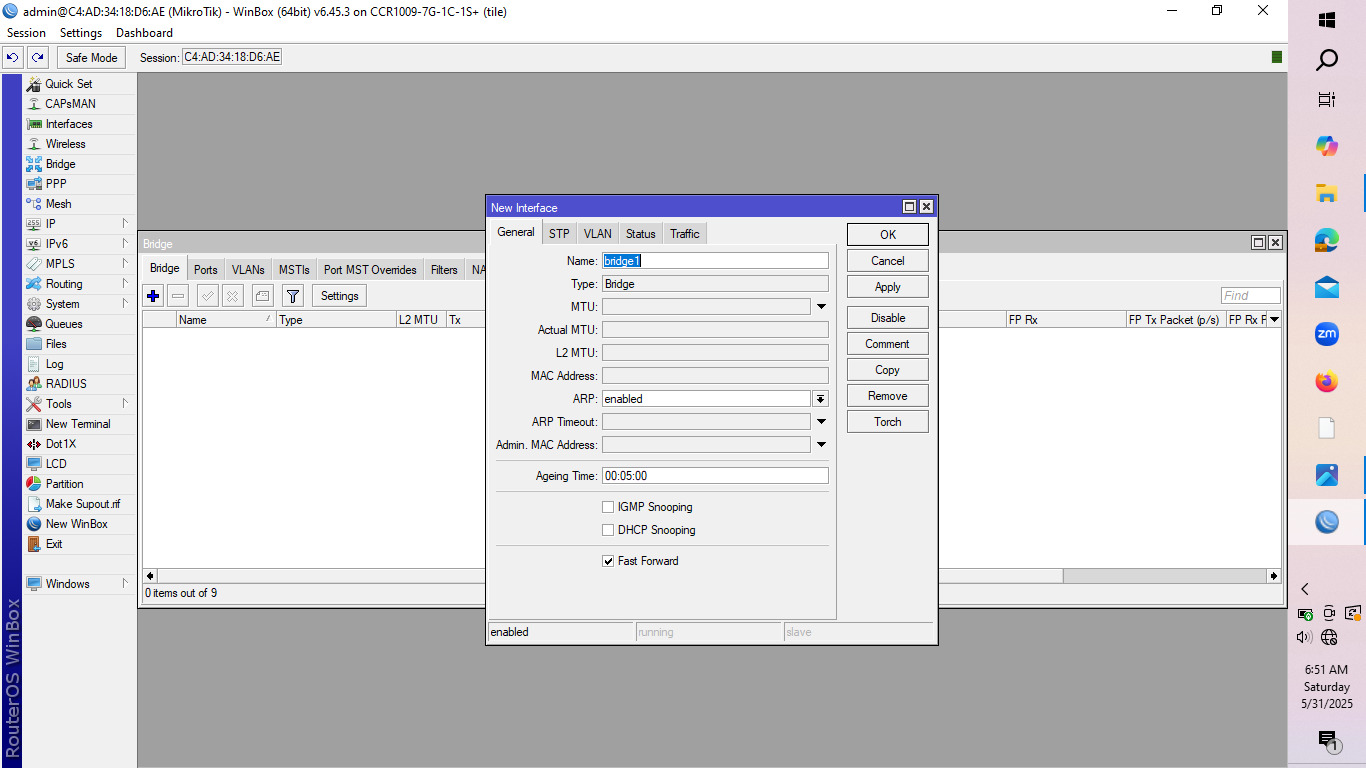
\includegraphics[width=0.5\linewidth]{P1/img/gambar7a.jpeg}
        \caption{Menetapkan konfigurasi Bridge pada Router B}
        \label{fig:mengkonfigurasikan-bridge-router-B}
    \end{figure}

    \begin{figure}[H]
        \centering
        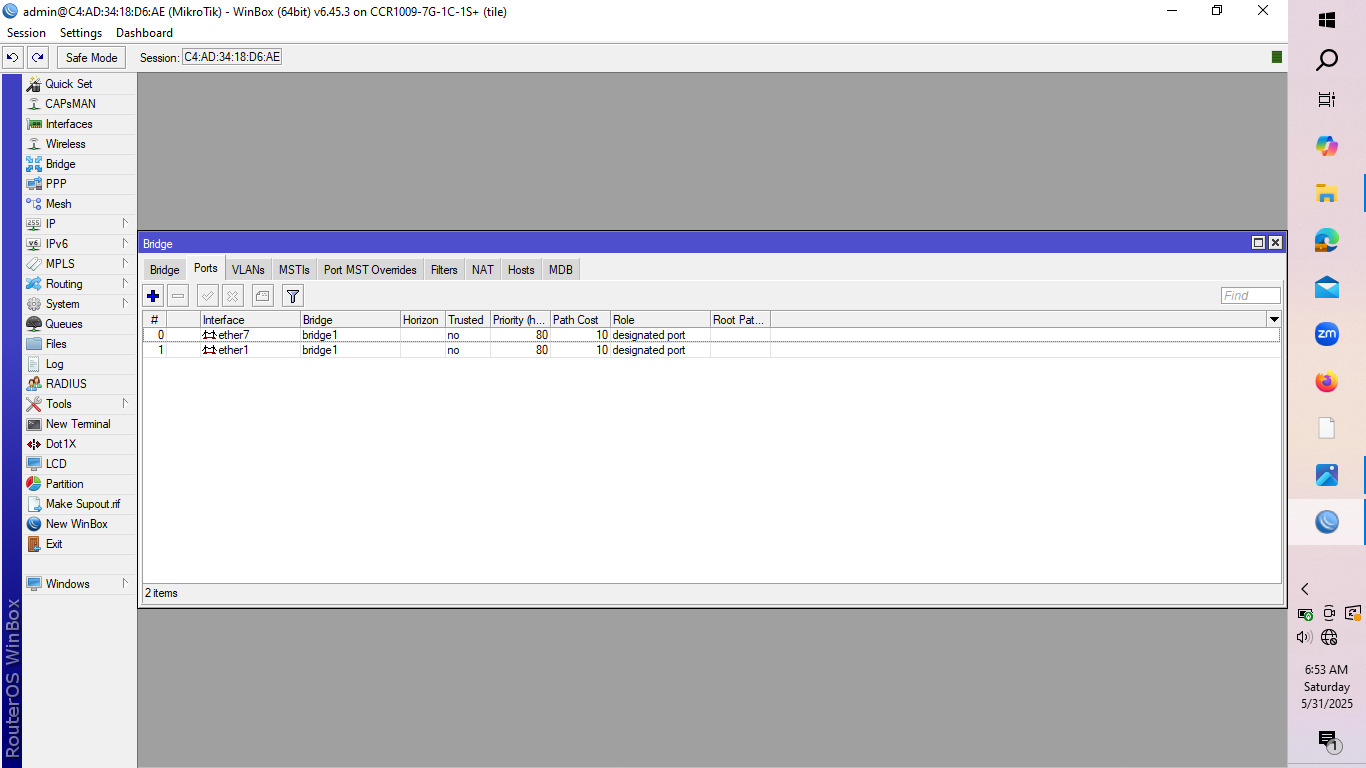
\includegraphics[width=0.5\linewidth]{P1/img/gambar7b.jpeg}
        \caption{Melakukan konfigurasi Bridge di Router B}
        \label{fig:mengkonfigurasikan-bridge-router-B}  
    \end{figure}
    \item Konfigurasi IP dilakukan lewat command prompt
    \begin{figure}[H]
        \centering
        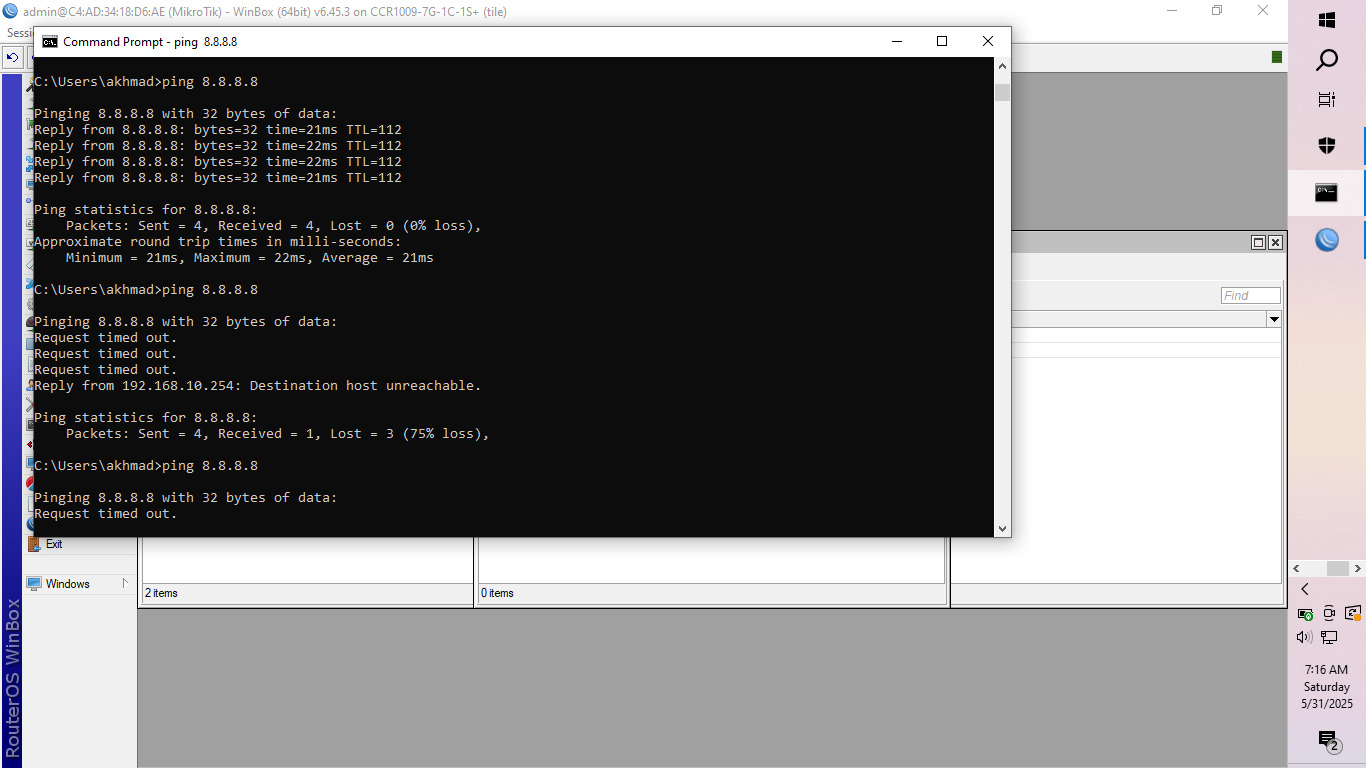
\includegraphics[width=0.5\linewidth]{P1/img/gambar8a.jpeg}
        \caption{Pengujian ping dalam kondisi firewall aktif}
        \label{fig:ping-saat-firewall-aktif}
    \end{figure}

    \begin{figure}[H]
        \centering
        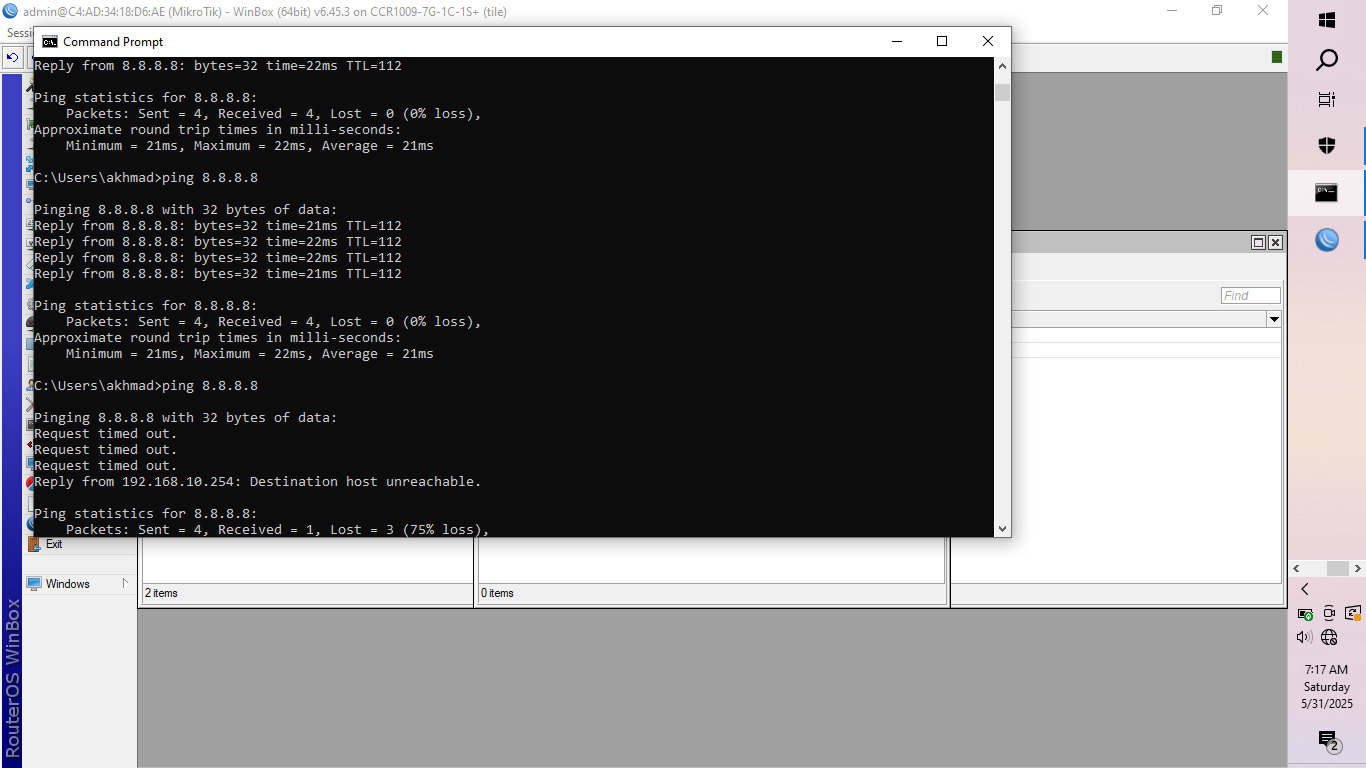
\includegraphics[width=0.5\linewidth]{P1/img/gambar8b.jpeg}
        \caption{Pengujian ping dalam kondisi firewall tidak aktif}
        \label{fig:ping-saat-firewall-tidak-aktif}
    \end{figure}

\end{enumerate}

\section{Analisis Hasil Percobaan}
Setelah melakukan percobaan, diperoleh hasil bahwa terdapat perbedaan perilaku jaringan ketika firewall dalam keadaan aktif dan tidak aktif. Saat firewall diaktifkan dan diberi aturan tertentu, proses ping tidak dapat dilakukan. Sebaliknya, ketika firewall dinonaktifkan, ping berhasil dilakukan. Ini membuktikan bahwa firewall berperan dalam mengatur lalu lintas jaringan serta melindungi sistem dari akses yang tidak diinginkan.

Pada percobaan NAT (Network Address Translation), diperoleh bahwa NAT berfungsi untuk mengubah alamat IP pada paket data yang melewati router. Mekanisme ini memungkinkan beberapa perangkat dalam jaringan lokal menggunakan satu alamat IP publik secara bersama-sama. Selain menghemat penggunaan alamat IP publik, NAT juga memberikan tambahan keamanan dengan menyembunyikan alamat IP internal dari paparan langsung ke jaringan publik.

\section{Hasil Tugas Modul}
    \begin{figure}[H]
        \centering
        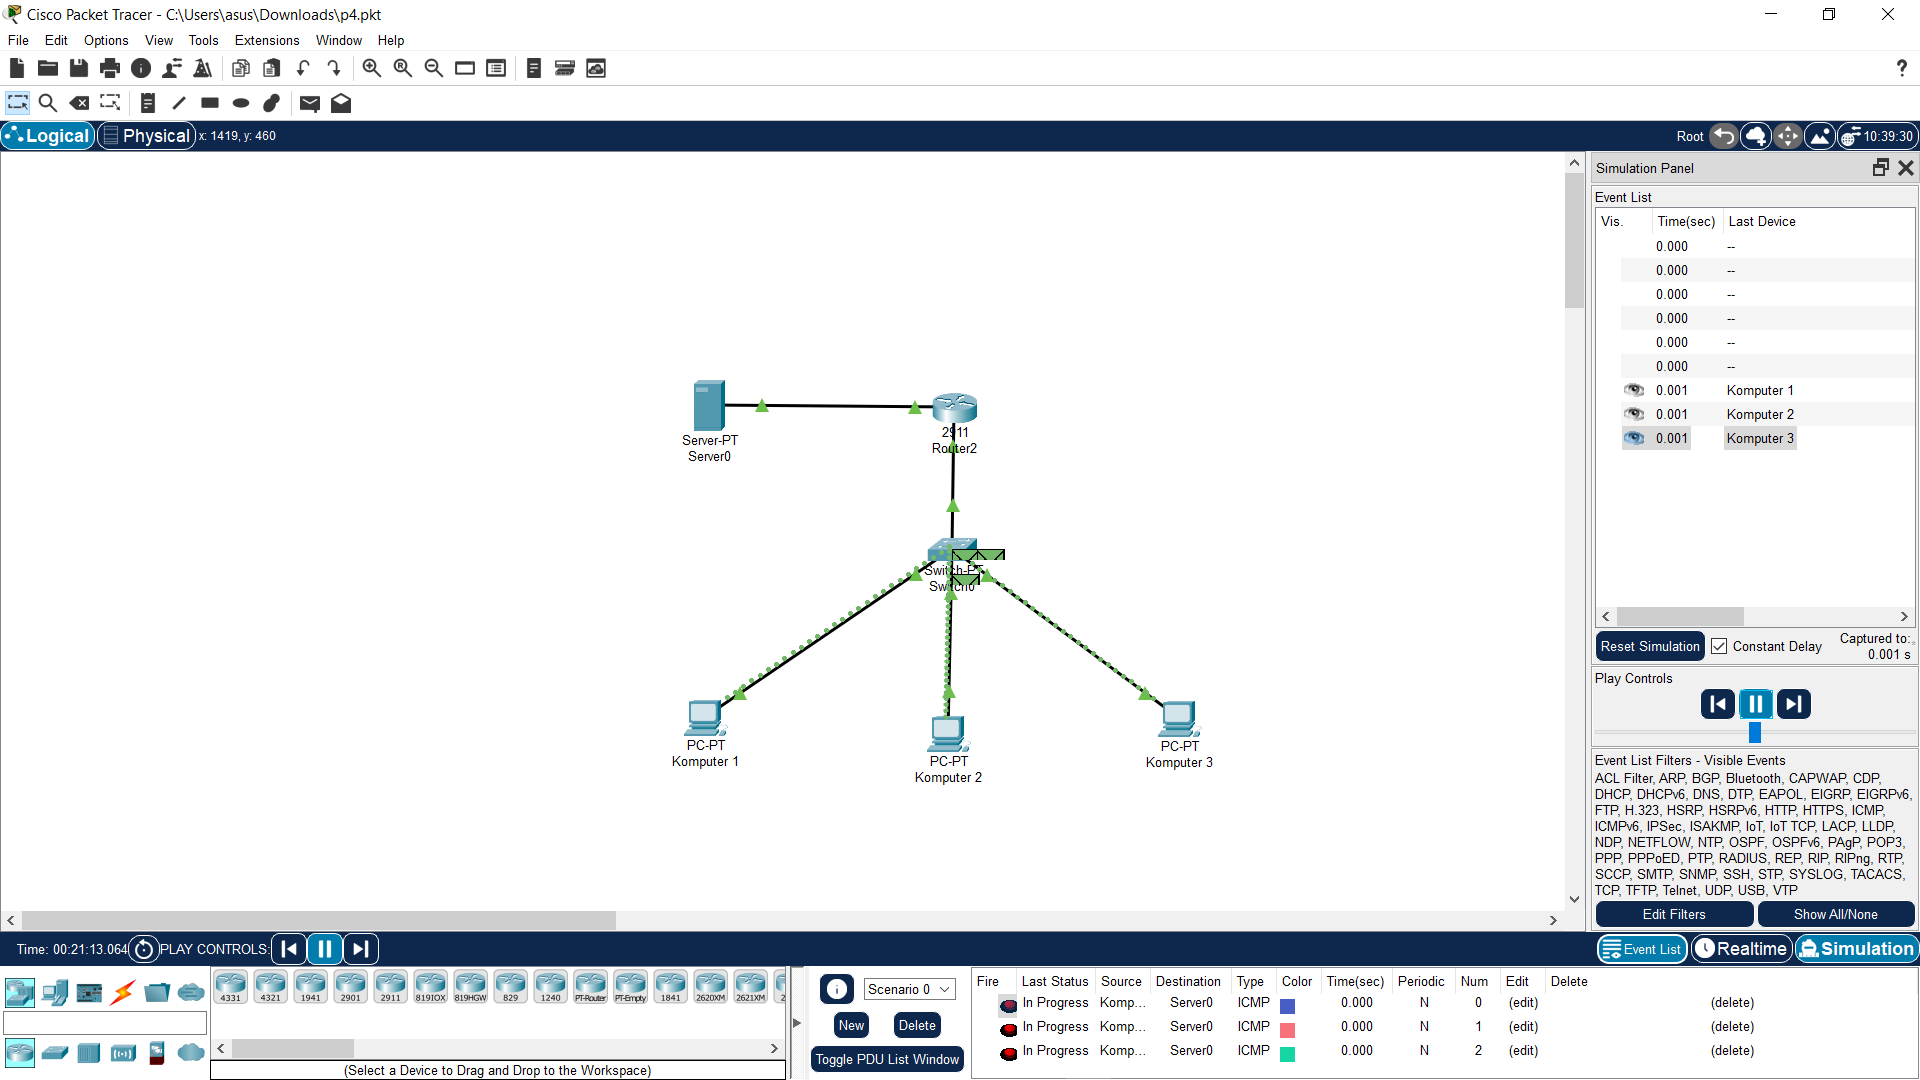
\includegraphics[width=0.5\linewidth]{P1/img/topologi.png}
        \caption{Topologi}
        \label{fig:gambar}
    \end{figure}

    \begin{figure}[H]
        \centering
        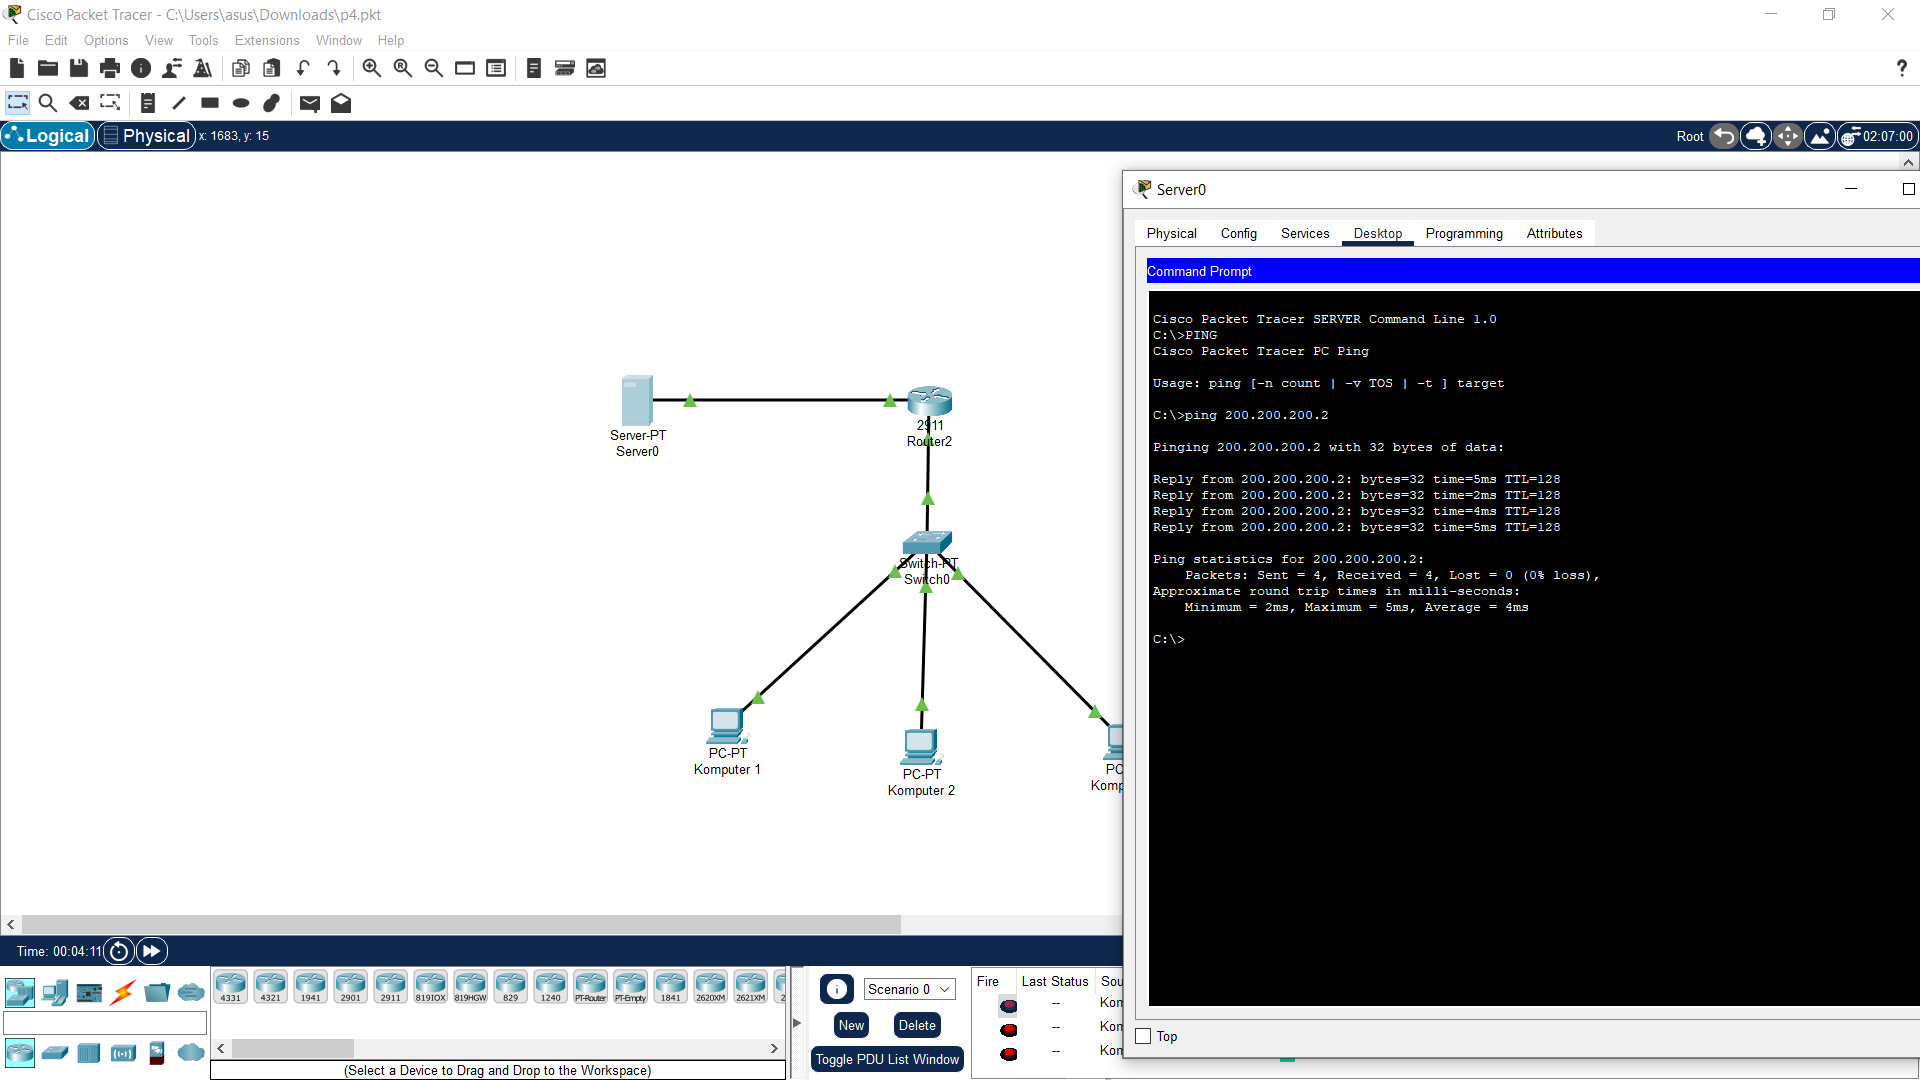
\includegraphics[width=0.5\linewidth]{P1/img/konfig.png}
        \caption{Konfigurasi}
        \label{fig:gambar}
    \end{figure}

    \begin{figure}[H]
        \centering
        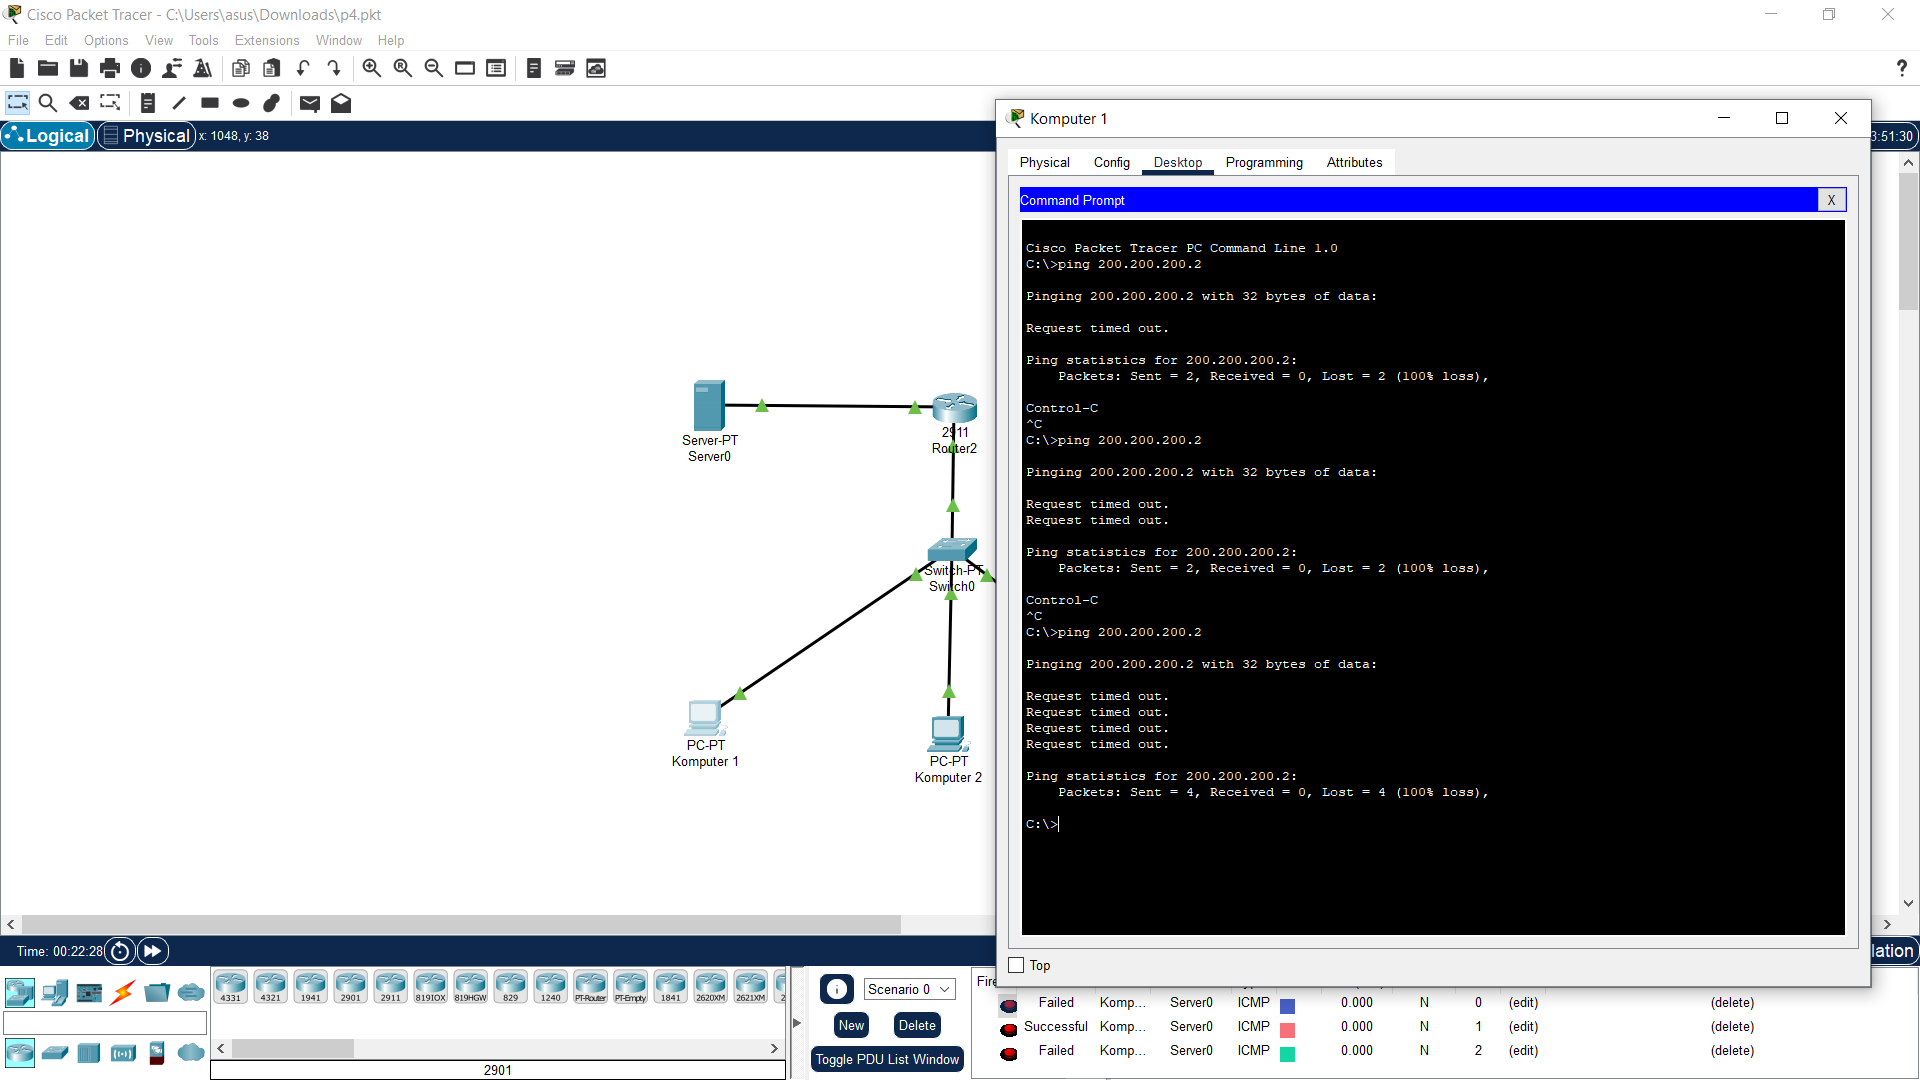
\includegraphics[width=0.5\linewidth]{P1/img/pingpc1.png}
        \caption{Melakukan ping dari PC 1 ke server}
        \label{fig:gambar}
    \end{figure}

    \begin{figure}[H]
        \centering
        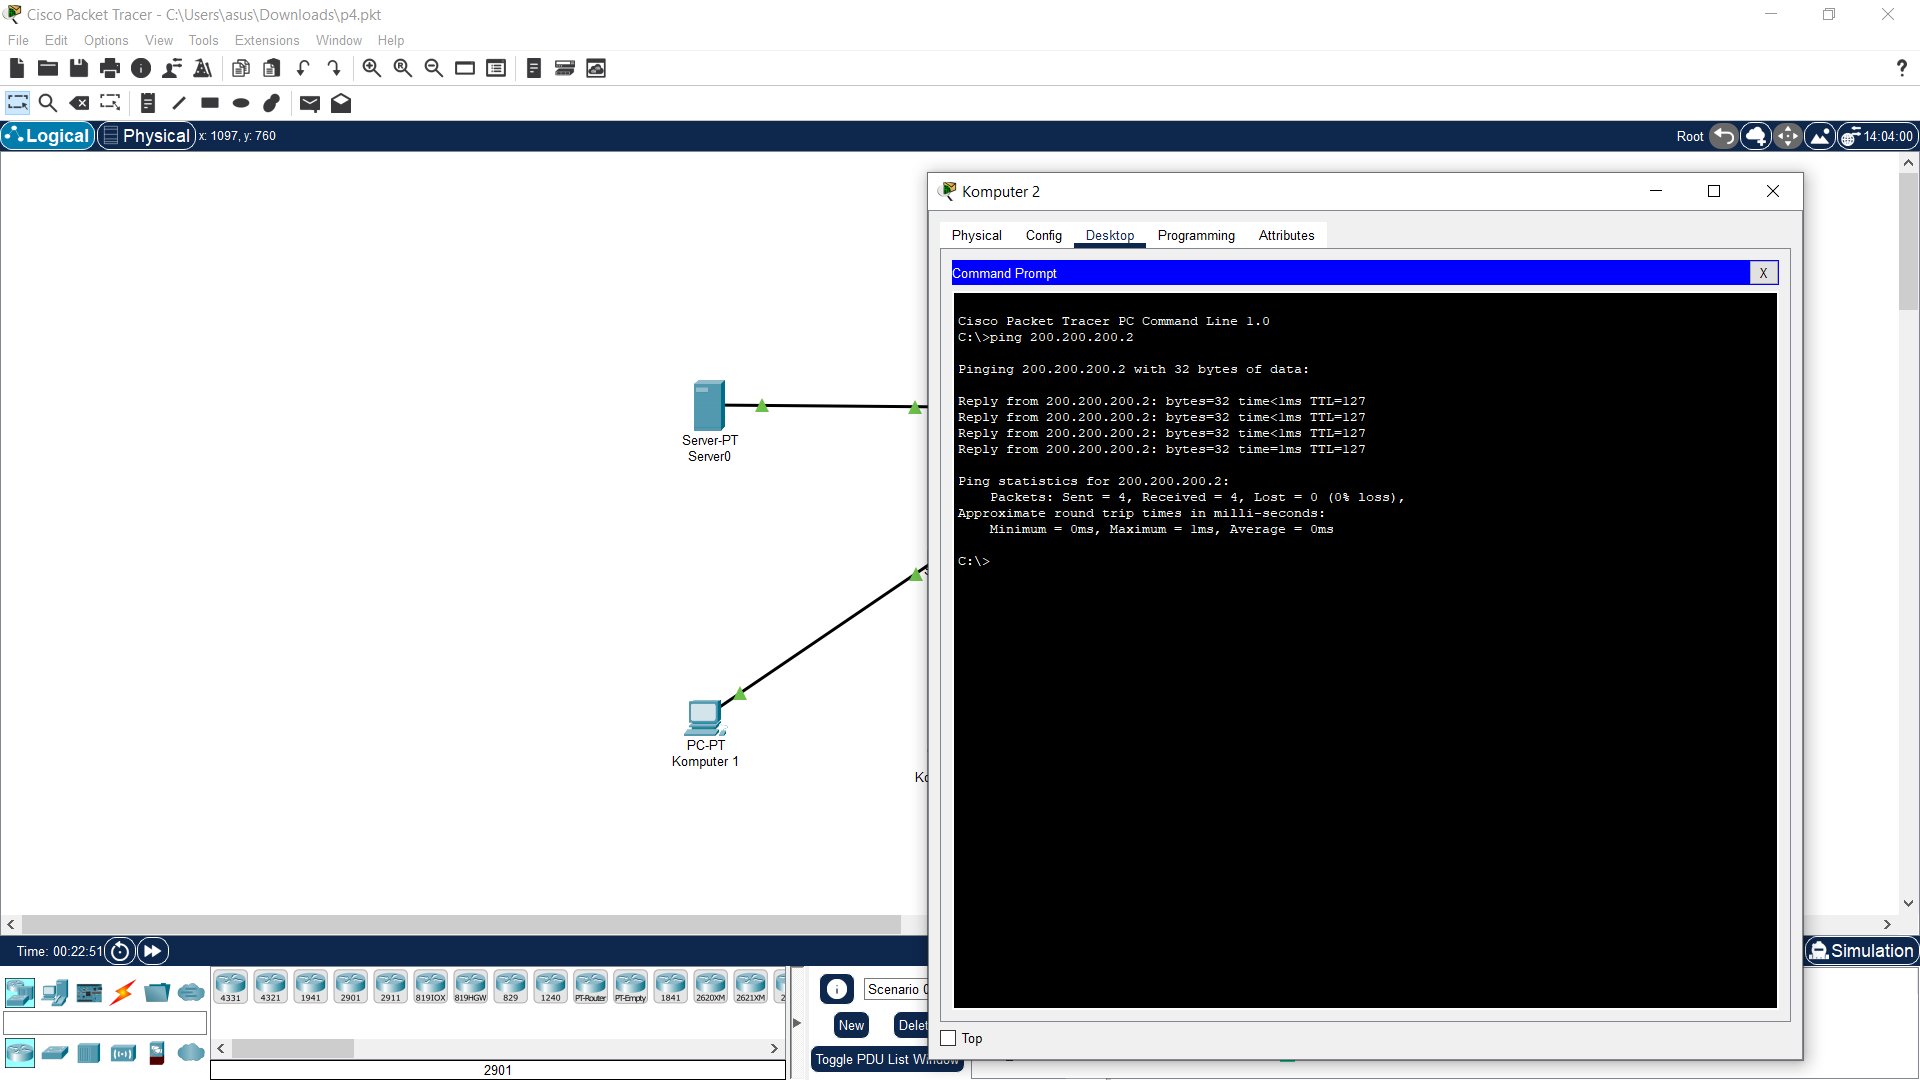
\includegraphics[width=0.5\linewidth]{P1/img/pingpc2.png}
        \caption{Melakukan ping dari PC 2 ke server}
        \label{fig:gambar}
    \end{figure}

    \begin{figure}[H]
        \centering
        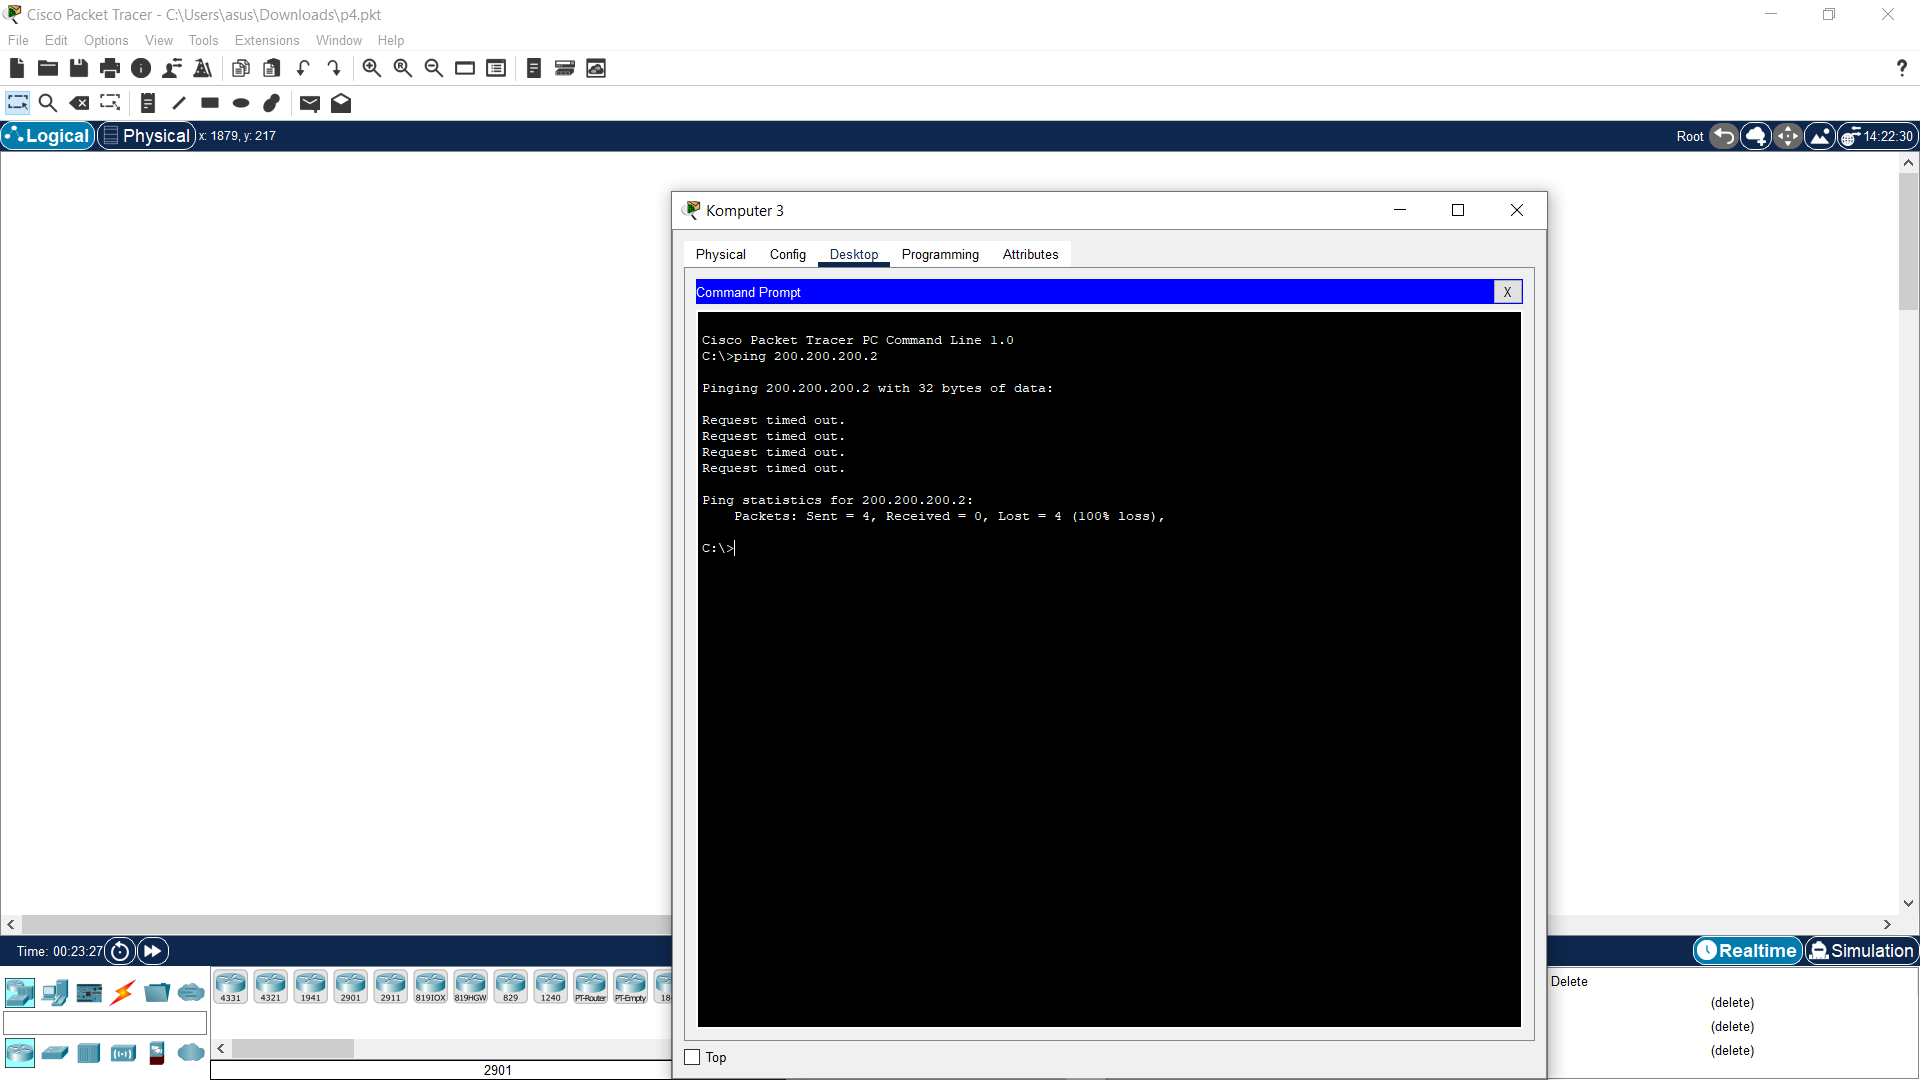
\includegraphics[width=0.5\linewidth]{P1/img/pingpc3.png}
        \caption{Melakukan ping dari PC 3 ke server}
        \label{fig:gambar}
    \end{figure}

\section{Kesimpulan}
Berdasarkan hasil praktikum, dapat disimpulkan bahwa firewall memiliki peran krusial dalam mengontrol dan melindungi lalu lintas jaringan melalui penerapan sejumlah aturan yang menentukan apakah suatu akses diizinkan atau ditolak. Di sisi lain, NAT berfungsi untuk menghemat penggunaan alamat IP publik dengan mengubah alamat IP lokal menjadi alamat IP publik, serta memungkinkan banyak perangkat dalam jaringan lokal untuk terhubung ke internet.

\section{Lampiran}
\subsection{Dokumentasi saat praktikum}
    \begin{figure}[H]
        \centering
        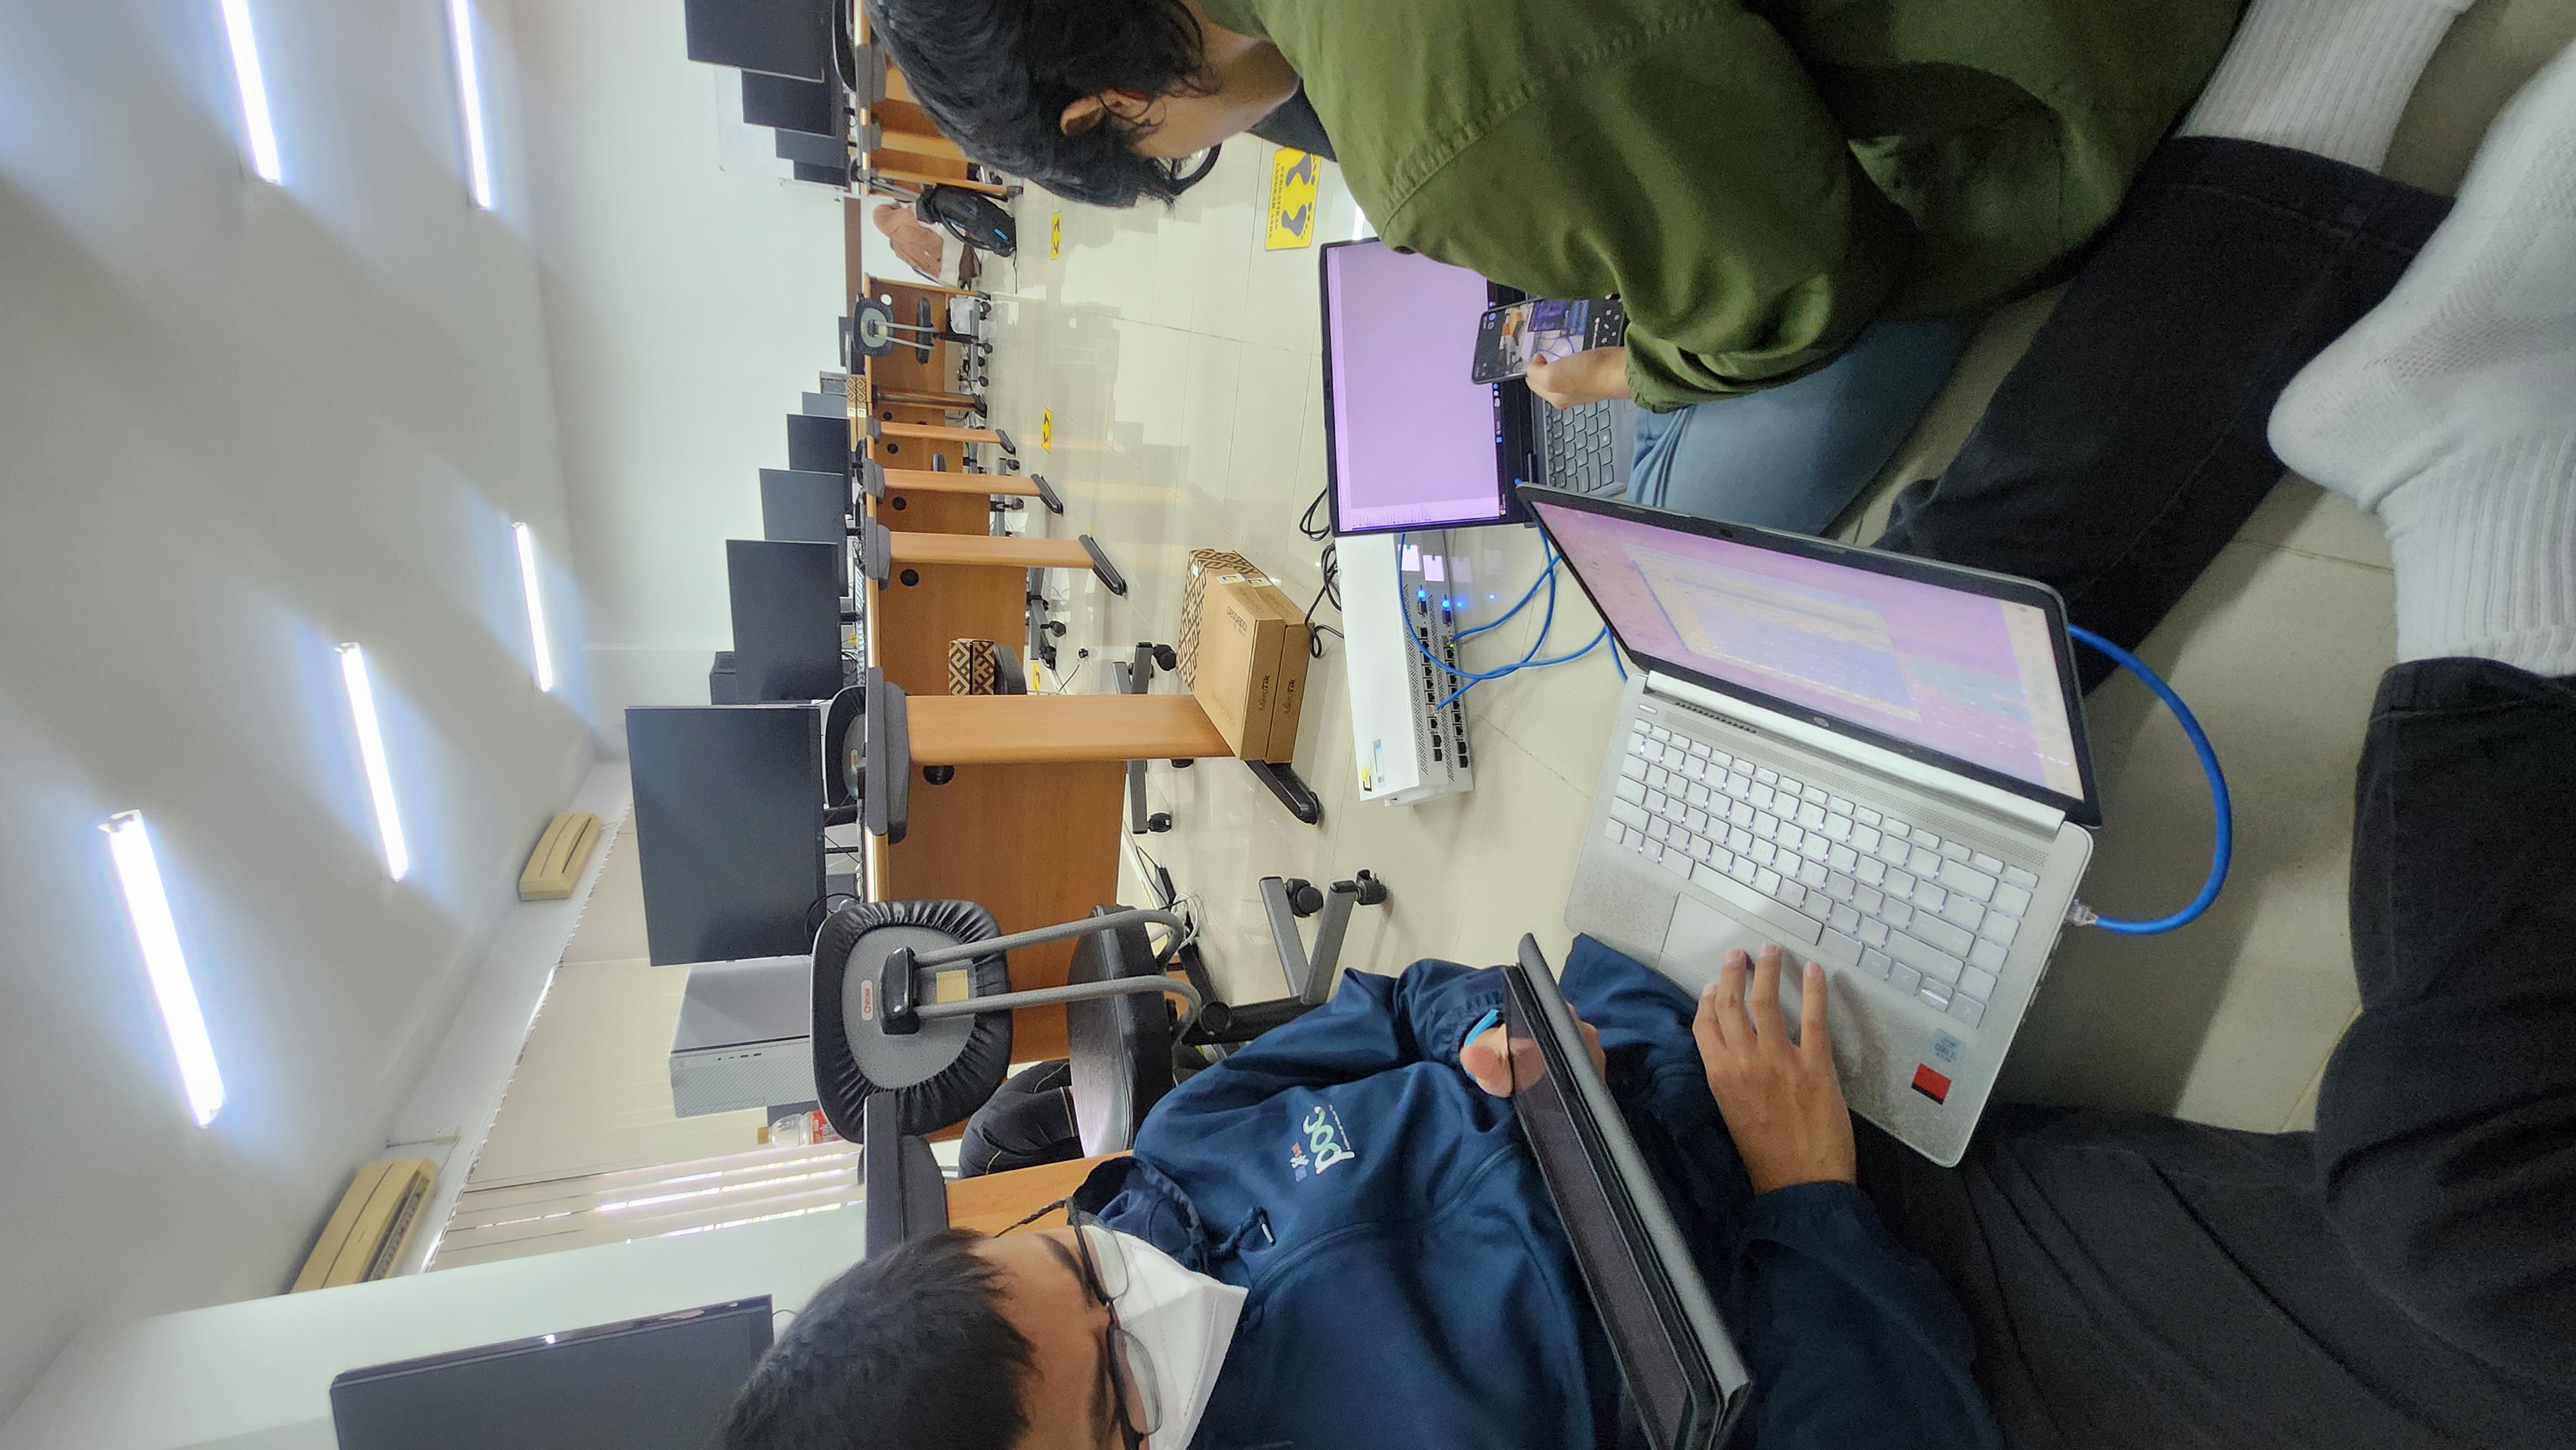
\includegraphics[width=0.5\linewidth]{P1/img/dokum.jpg}
        \label{fig:gambar}
    \end{figure}